\documentclass{article}
\usepackage[margin=1in]{geometry}
\usepackage{amsmath,amsthm,amssymb}
\usepackage{bbm,enumerate,mathtools}
\usepackage{tikz,pgfplots}
\usepackage{chessboard}
\usepackage[hidelinks]{hyperref}
\usepackage{multicol} % Problem 35
\usepackage{xstring} % Difficulty command
\usetikzlibrary{shapes.geometric}

\newenvironment{question}{\begin{trivlist}\item[\textbf{Question.}]}{\end{trivlist}}
\newenvironment{note}{\begin{trivlist}\item[\textbf{Note.}]}{\end{trivlist}}
\newenvironment{references}{\begin{trivlist}\item[\textbf{References.}]}{\end{trivlist}}
\newenvironment{related}{\begin{trivlist}\item[\textbf{Related.}]\end{trivlist}\begin{enumerate}}{\end{enumerate}}

\newcommand\score[1]{
\pgfmathsetmacro\pgfxa{#1+1}
\tikzstyle{scorestars}=[
  star,
  star points=5,
  star point ratio=2.25,
  draw,
  inner sep=3pt,
  anchor=outer point 5
]
  \begin{tikzpicture}[baseline]
    \draw[opacity=0] (0,-0.5) rectangle (0,0.2); % Workaround for whitespace at the bottom.
    \foreach \i in {1,...,4} {
      \pgfmathparse{(\i<=#1?"yellow":"gray")}
      \edef\starcolor{\pgfmathresult}
      \draw (\i*4.5ex,0) node[name=star\i,scorestars,fill=\starcolor]  {};
    }
  \end{tikzpicture}
}

\newcommand{\difficulty}[1]{%
  \IfEqCase{#1}{%
      {1}{
        
\begin{tikzpicture}[scale=0.7, baseline=0.9mm]%
          \definecolor{slopegreen}{rgb}{0.0, 0.5, 0.0}%
          \fill[slopegreen] (0.5,0.5) circle (0.5);%
        \end{tikzpicture}%
      }%
      {2}{
        
\begin{tikzpicture}[scale=0.7, baseline=0.9mm]%
          \definecolor{slopeblue}{rgb}{0.0, 0.44, 1.00}
          \fill[slopeblue] (0,0) rectangle (1,1);%
        \end{tikzpicture}%
      }%
      {3}{
\begin{tikzpicture}[scale=0.7, baseline=0.9mm]\fill (0,0.5)--(0.5, 0)--(1,0.5)--(0.5,1)--cycle; \end{tikzpicture}}%
      {4}{
\begin{tikzpicture}[scale=0.7, baseline=0.9mm]\fill (0.25,0)--(0,0.5)--(0.25,1)--(0.5,0.5)--cycle; \fill (0.75,0)--(0.5,0.5)--(0.75,1)--(1,0.5)--cycle;\end{tikzpicture}}%
      % you can add more cases here as desired
  }[\PackageError{difficulty}{Undefined difficulty level: #1}{}]%
}%
\newcommand{\rating}[2]{\difficulty{#1}\\\score{#2}\\}


\begin{document}
  Consider the art gallery problem on all ``museum''-equivalence classes of polygons.
  \begin{figure}[ht!]
    \centering
    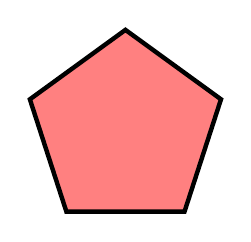
\begin{tikzpicture}[scale=1.5]
      \draw[ultra thick, fill=red!50] (1,0)
        --(0,0)
        --({-cos(72)}, {sin(72)})
        --({-cos(72)+cos(36)}, {sin(72)+sin(36)})
        --({1+cos(72)}, {sin(72)})
        --cycle;
    \end{tikzpicture}\hspace{0.5cm}
    
\begin{tikzpicture}[scale=1.5]
      \draw[ultra thick, fill=orange!50] (0,0)--(1.54/2,1.54/2)--(1.54,0)--(1.54,1.54)--(0,1.54)--cycle;
    \end{tikzpicture}\hspace{0.5cm}
    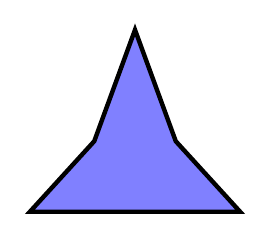
\begin{tikzpicture}[scale=1.5]
      \draw[ultra thick, fill=blue!50] (0,0)
        --({1.78/4 + 0.1}, {1.78*sqrt(3)/4 - 0.1*sqrt(3)})
        --(1.78/2,1.54)
        --({3*1.78/4 - 0.1}, {1.78*sqrt(3)/4 - 0.1*sqrt(3)})
        --(1.78,0)
        --cycle;
    \end{tikzpicture}\hspace{0.5cm}
    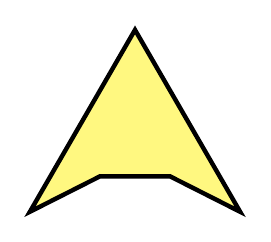
\begin{tikzpicture}[scale=1.5]
      \draw[ultra thick, fill=yellow!50] (0,0)
        --(1.78/2,1.54)
        --(1.78,0)
        --({2*1.78/3}, 0.3)
        --({1.78/3}, 0.3)
        --cycle;
    \end{tikzpicture}\hspace{0.5cm}
    
\begin{tikzpicture}[scale=1.5]
      \draw[ultra thick, fill=green!50] (0,0)
        --(1.78/2,1.54)
        --(1.78,0)
        --({1.78/2}, 0.6)
        --({3*1.78/8}, 0.3)
        --cycle;
    \end{tikzpicture}
    \caption{
      The $a(5) = 5$ concavity classes on the pentagon.
    }
  \end{figure}
  \begin{question}
    If each polygon is a museum, how many guards are required to patrol the museum?
  \end{question}

  \begin{related}
    \item What if guards are stationed at a corner in the polygon?
    \item What if guards are allowed to patrol along a wall?
    \item What if the polygons are on a torus or cylinder?
    \item What if the polygons are orthogonal (i.e. each wall meets at a right angle)?
    \item What if the guards must patrol the outside of the polygon?
    \item How many equivalence classes of museums exist? For example, the
    following museums are distinct, because the first requires two guards, and
    the second requires only one.\\~\\
    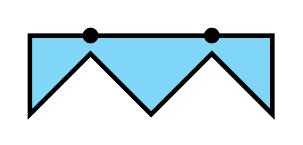
\begin{tikzpicture}
      \draw[ultra thick, fill=cyan!50] (0,0)--(1.54/2, 1.54/2)--(1.54,0)--(3/2*1.54,1.54/2)--(2*1.54,0)--(2*1.54,1)--(0,1)--cycle;
      \fill (1.54/2, 1) circle (0.1);
      \fill (3/2*1.54, 1) circle (0.1);
    \end{tikzpicture}\hspace{0.5cm}
    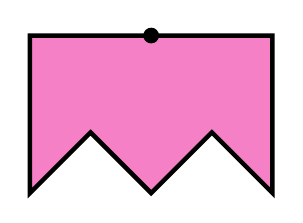
\begin{tikzpicture}
      \draw[ultra thick, fill=magenta!50] (0,0)--(1.54/2, 1.54/2)--(1.54,0)--(3/2*1.54,1.54/2)--(2*1.54,0)--(2*1.54,2)--(0,2)--cycle;
      \fill (1.54, 2) circle (0.1);
    \end{tikzpicture}
  \end{related}
  \begin{references}
    \item Problem 61.
    \item \url{https://en.wikipedia.org/wiki/Art_gallery_problem}
  \end{references}
\end{document}
